\scanpage{52}
% archive sheet number: 51

\deleted{\unsure{NB}} des deux arcs \inserted{ouverts} déterminés par $s,t$ sur $\partial F$, il y a au moins un pt critique

d) \uline{Relation entre} sommets critiques \deleted{\unsure{de}} sur $F$ et sur $F'=\sigma_a(F)$ $a$ une \uline{grande arête} sur $\partial F$. \unsure{OPS|UPS} que $\varepsilon_F(a)=+1$ (quitte à intervertir les rôles de $F$ et $F'$). On a donc ceci : Soit \deleted{$s$ le pt critique sur $a$,} \inserted{$t$ l'antipodique de $s$, qui est critique,} $u,v$ les deux pts critiques les plus voisins de \deleted{$\partial F$} \unsure{$t|s$}, de part et d'autre de $s$, \deleted{\unsure{$s$}} $\beta=\widehat{u\unsure{t|s}v}$ l'arc correspondant \inserted{de $\partial F$,} d'extrémités $u,v$ contenant $s$. Considérons \deleted{$\beta=$} l'autre arc d'extrémités $u$ et $v$, soit $\alpha$. \deleted{Soient} (NB, on a $u,v$ sur \deleted{deux} arcs \inserted{ouverts} distincts déterminés par $s,t$ sur $\partial F$, \deleted{donc} et $u\ne v$, donc $s\in\deleted{\beta}\alpha$, de façon précise $\alpha=\widehat{usv}$). \deleted{Soient} \inserted{$s'=s$,} $t',u',v'$ \deleted{leurs} transformés de $s,t,u,v$ par $\sigma_a$.

\figure{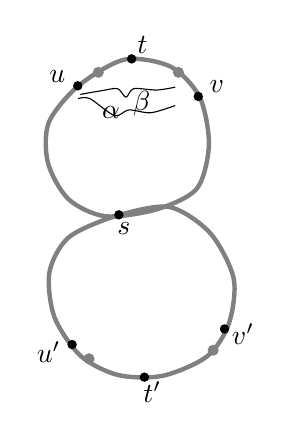
\begin{tikzpicture}[x=0.009cm,y=-0.009cm,line cap=round,line join=round]
\draw[gray,line width=1.6pt] plot[smooth cycle] coordinates {(55,47) (120,10) (185,20) (226,63) (239,130) (222,192) (166,221) (93,231) (41,207) (12,156) (13,99)};
\draw[gray,line width=1.6pt] plot[smooth cycle] coordinates {(107,231) (183,218) (241,255) (274,319) (267,383) (236,429) (174,456) (111,455) (58,428) (21,373) (14,310) (41,261)};
\fill[black] (54,47) circle [radius=1.7pt];
\fill[black] (130,9) circle [radius=1.7pt];
\fill[black] (224,62) circle [radius=1.7pt];
\fill[black] (112,229) circle [radius=1.7pt];
\fill[black] (46,412) circle [radius=1.7pt];
\fill[black] (261,390) circle [radius=1.7pt];
\fill[black] (148,458) circle [radius=1.7pt];
\fill[gray] (83,28) circle [radius=2pt];
\fill[gray] (196,28) circle [radius=2pt];
\fill[gray] (70,432) circle [radius=2pt];
\fill[gray] (245,420) circle [radius=2pt];
\node at (25,34) {$u$};
\node at (145,-10) {$t$};
\node at (250,48) {$v$};
\node at (119,249) {$s$};
\node at (13,423) {$u'$};
\node at (287,397) {$v'$};
\node at (159,479) {$t'$};
\draw[thin] plot[smooth] coordinates {(58,59) (87,54) (110,51) (122,63) (133,51) (165,53) (191,49)};
\node at (144,72) {$\beta$};
\draw[thin] plot[smooth] coordinates {(55,65) (71,65) (106,89) (126,81) (157,85) (191,75)};
\node at (101,84) {$\unsure{\alpha}$};
\end{tikzpicture}}

Alors

a) \deleted{\unsure{$C_K$}} $\sigma_a$ \uline{induit une bijection entre $C_K\cap\alpha$ et $C_K\cap\alpha'$.} \deleted{Il en résulte, avec la relation 1) ci-dessus, que} Si $x$ et $x'$ se correspondent par $\sigma$, on a $\varepsilon_F(x)=\varepsilon_{F'}(x')$, sauf si $x=s$, donc $x'=s$, (auquel cas on a $\varepsilon_{F'}(x)=-\varepsilon_F(x)$)

b) On a $t'\notin C_K$ ; \deleted{l'intersection} \inserted{on a} $\operatorname{Card}(\mathring{\beta}'\cap C_K)$ \deleted{\unsure{$\in\{0,1\}$}} $\in\{0,1,2\}$. (\deleted{\unsure{On|Donc}} \inserted{ou si l'\inserted{indice} de $F$ resp $F'$ est $N$ resp $N'$, on a $N'\in\{N-1,N,N+1\}$.} \deleted{\unsure{tels} Si} Si $x\in\mathring{\beta}'\cap C_K$, on a $\varepsilon_F(x)=-1$

\uline{Cor.} Considérons les antipodiques $u^*,v^*$ de $u,v$ sur $\partial F$, et l'arc $\beta^*=\widehat{u^*sv^*}$, \deleted{Alors} alors sur cet arc il n'y a pas de pts critiques de signe $\pm1$

\uline{En résumé} \quad Soit $x\in S_K\cap\partial F$, \deleted{Pour les sommets de $s$} $x'\deleted{\unsure{=}}=\sigma_a(F)$, alors $x'$ est critique sss $a$ l'est, et $x$ et $x'$ \unsure{x|ont} $=$ indice sauf dans les cas suivants

a) $x=s$, auquel cas $\varepsilon_{F'}(x)=-\varepsilon_F(x')$

b) $x=t$, auquel cas \deleted{\unsure{un}} $x$ est critique d'indice $+1$, \unsure{$x''$|$x'$} non critique

(Ceci permet de distinguer \deleted{qui est} \inserted{lequel} des deux faces $F,F'$ est ``\deleted{\unsure{générique|généreux}}\inserted{spécialisée}'' par r. à l'autre, en termes de la position de l'arc critique \deleted{\unsure{$t$}} sur $a$ et ses \deleted{\unsure{d}}es antipodiques sur $\partial F,\partial F'$)

c) $x\in\overset{\circ}{\widehat{utv}}=\beta^\circ$, avec $x\ne t$ i.e. $x'\ne t'$, alors $x$ non critique, alors qu'il peut exister 1 resp 2 cas (au maximum) tels que $x'$ soit critique --- son indice est alors $-1$.
